\chapter{Evaluation}
\label{eval}

\section{Andere Systeme}

\subsection{Zookeeper}

\section{Benchmark}

\section{Ergebnisse}

\begin{figure}[t]
	\centering
	\begin{subfigure}[t]{0.45\textwidth}
		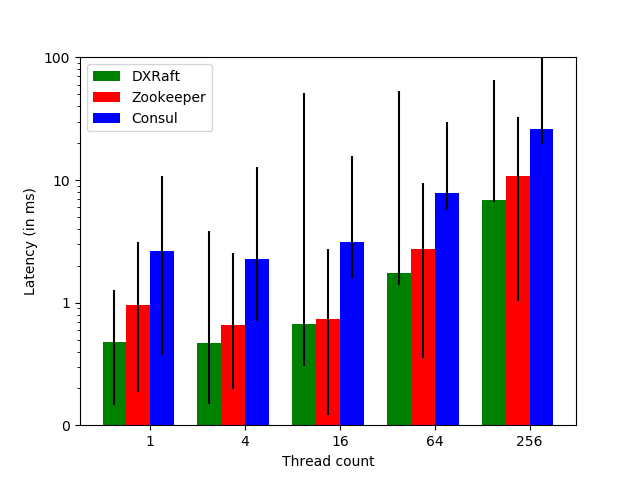
\includegraphics[width=\textwidth]{img/latency.png}
		\caption{Latenz.}
		\label{fig:latency}
	\end{subfigure}
	\begin{subfigure}[t]{0.45\textwidth}
		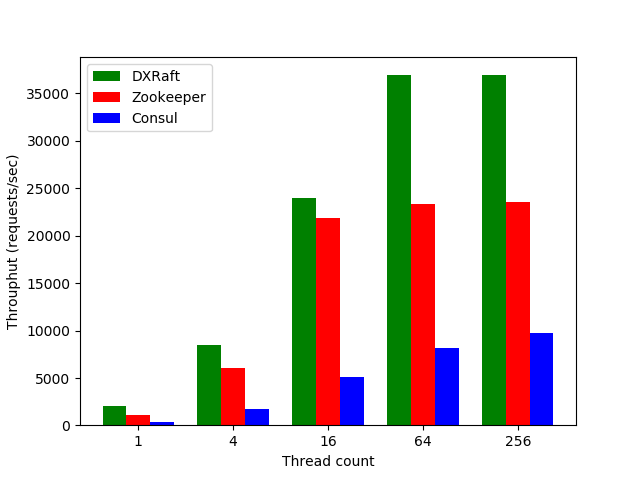
\includegraphics[width=\textwidth]{img/throughput.png}
		\caption{Durchsatz.}
		\label{fig:throughput}
	\end{subfigure}
	\caption{Benchmark mit einem Client und drei Server.}
\end{figure}

\begin{figure}[t]
	\centering
	\begin{subfigure}[t]{0.45\textwidth}
		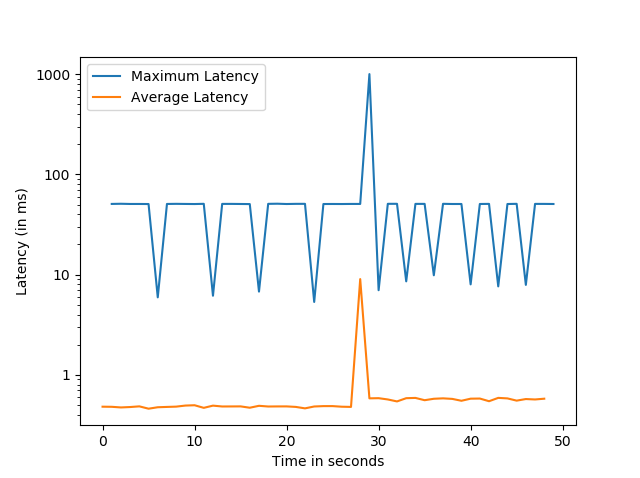
\includegraphics[width=\textwidth]{img/leader_crash_dxraft.png}
		\caption{DXRaft.}
	\end{subfigure}
	\begin{subfigure}[t]{0.45\textwidth}
		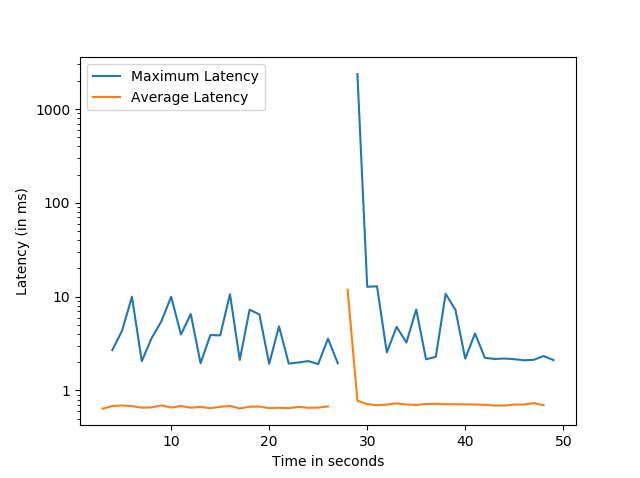
\includegraphics[width=\textwidth]{img/leader_crash_zk.png}
		\caption{Zookeeper.}
	\end{subfigure}
	\begin{subfigure}[t]{0.45\textwidth}
		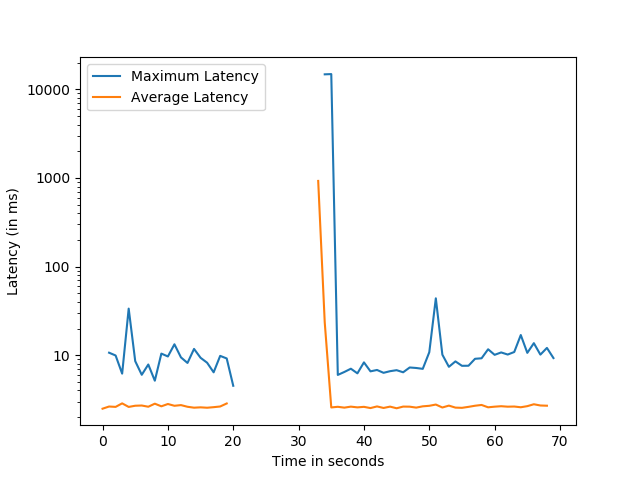
\includegraphics[width=\textwidth]{img/leader_crash_consul.png}
		\caption{Consul.}
	\end{subfigure}
	\caption{Latenz bei einem Leader-Crash.}
\end{figure}

\begin{figure}[t]
	\centering
	\begin{subfigure}[t]{1\textwidth}
		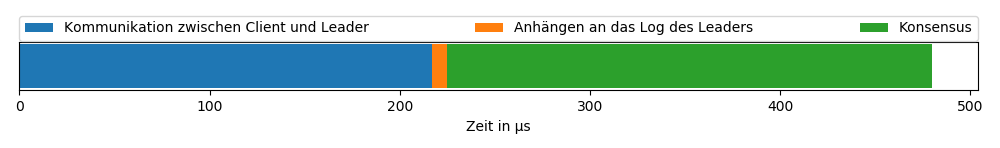
\includegraphics[width=\textwidth]{img/request_avg_timing.png}
		\caption{Durchschnittliche Anfrage.}
	\end{subfigure}
	\begin{subfigure}[t]{1\textwidth}
		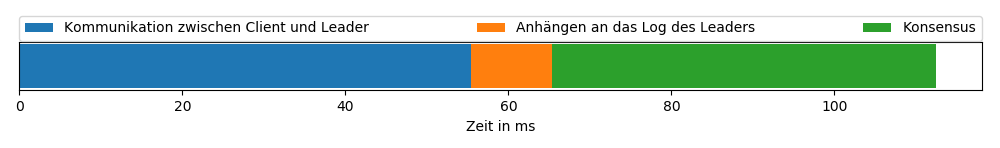
\includegraphics[width=\textwidth]{img/request_max_timing.png}
		\caption{Maximale Zeiten.}
	\end{subfigure}
	\begin{subfigure}[t]{1\textwidth}
		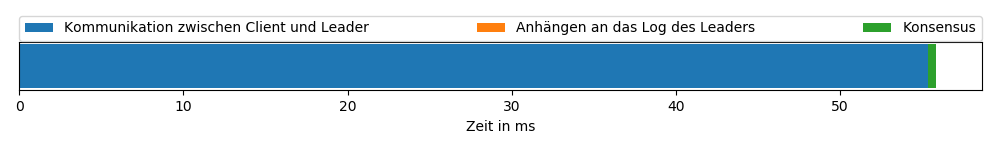
\includegraphics[width=\textwidth]{img/request_longest_timing.png}
		\caption{Längste Anfrage.}
	\end{subfigure}
\end{figure}